\documentclass{beamer}

\usepackage{beamerthemesplit}
\usepackage{tikz-uml}
%\usetheme{}

\title{Kolejka Projekt}
\subtitle{UML-Diagramm - Erster Entwurf}
\author{Gruppe A}
\date{\today}

\begin{document}
\maketitle
\frame{\tableofcontents[currentsection]}


\section{UML-Diagramme}
\begin{frame}
	\frametitle{Klassenbeziehungen - Überblick}
	\begin{center}		
		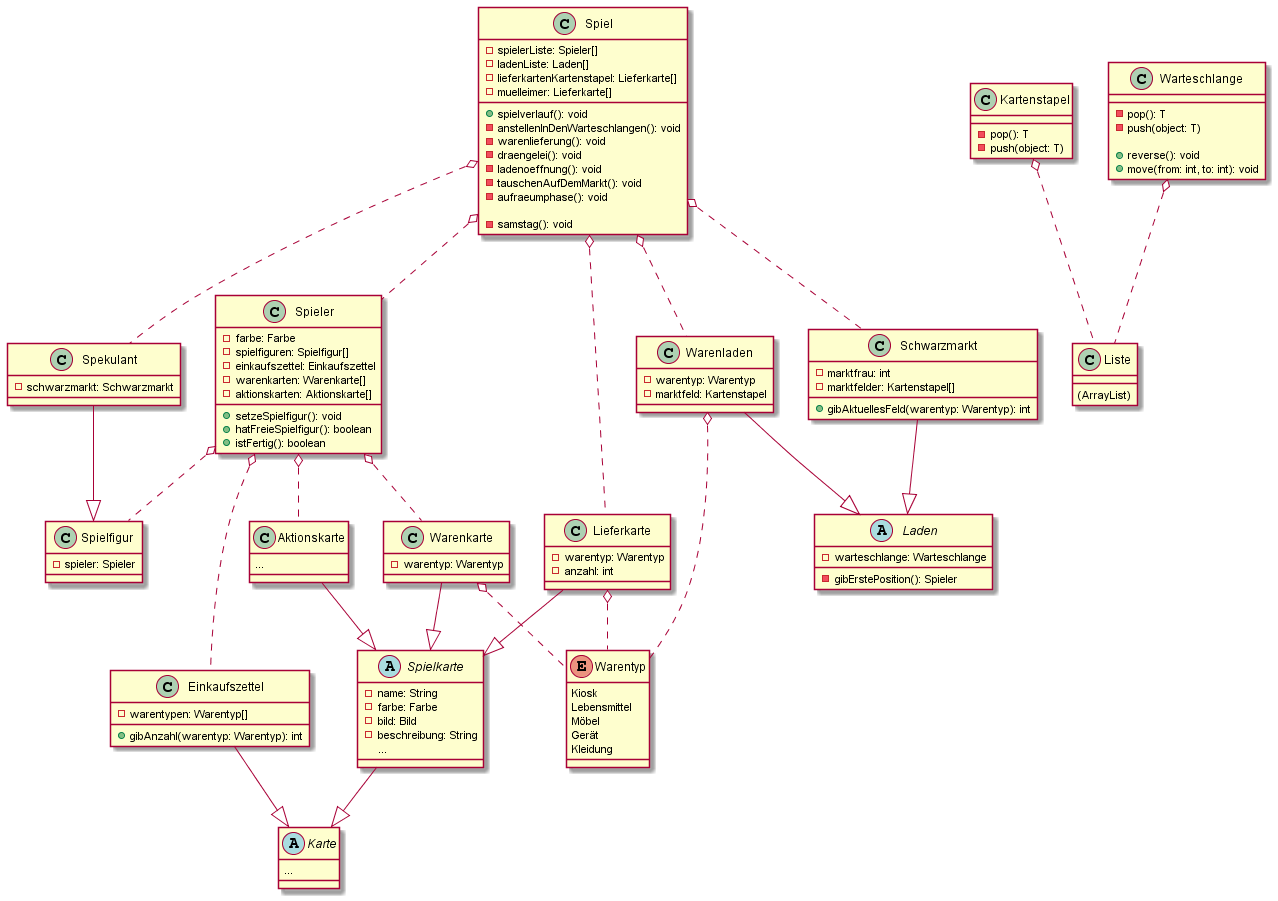
\includegraphics[width=1\textwidth]{../../diagrams/out/architecture_overview/architecture_overview.png}
	\end{center}
\end{frame}

\begin{frame}
	\frametitle{Klassen}
	\begin{center}		
		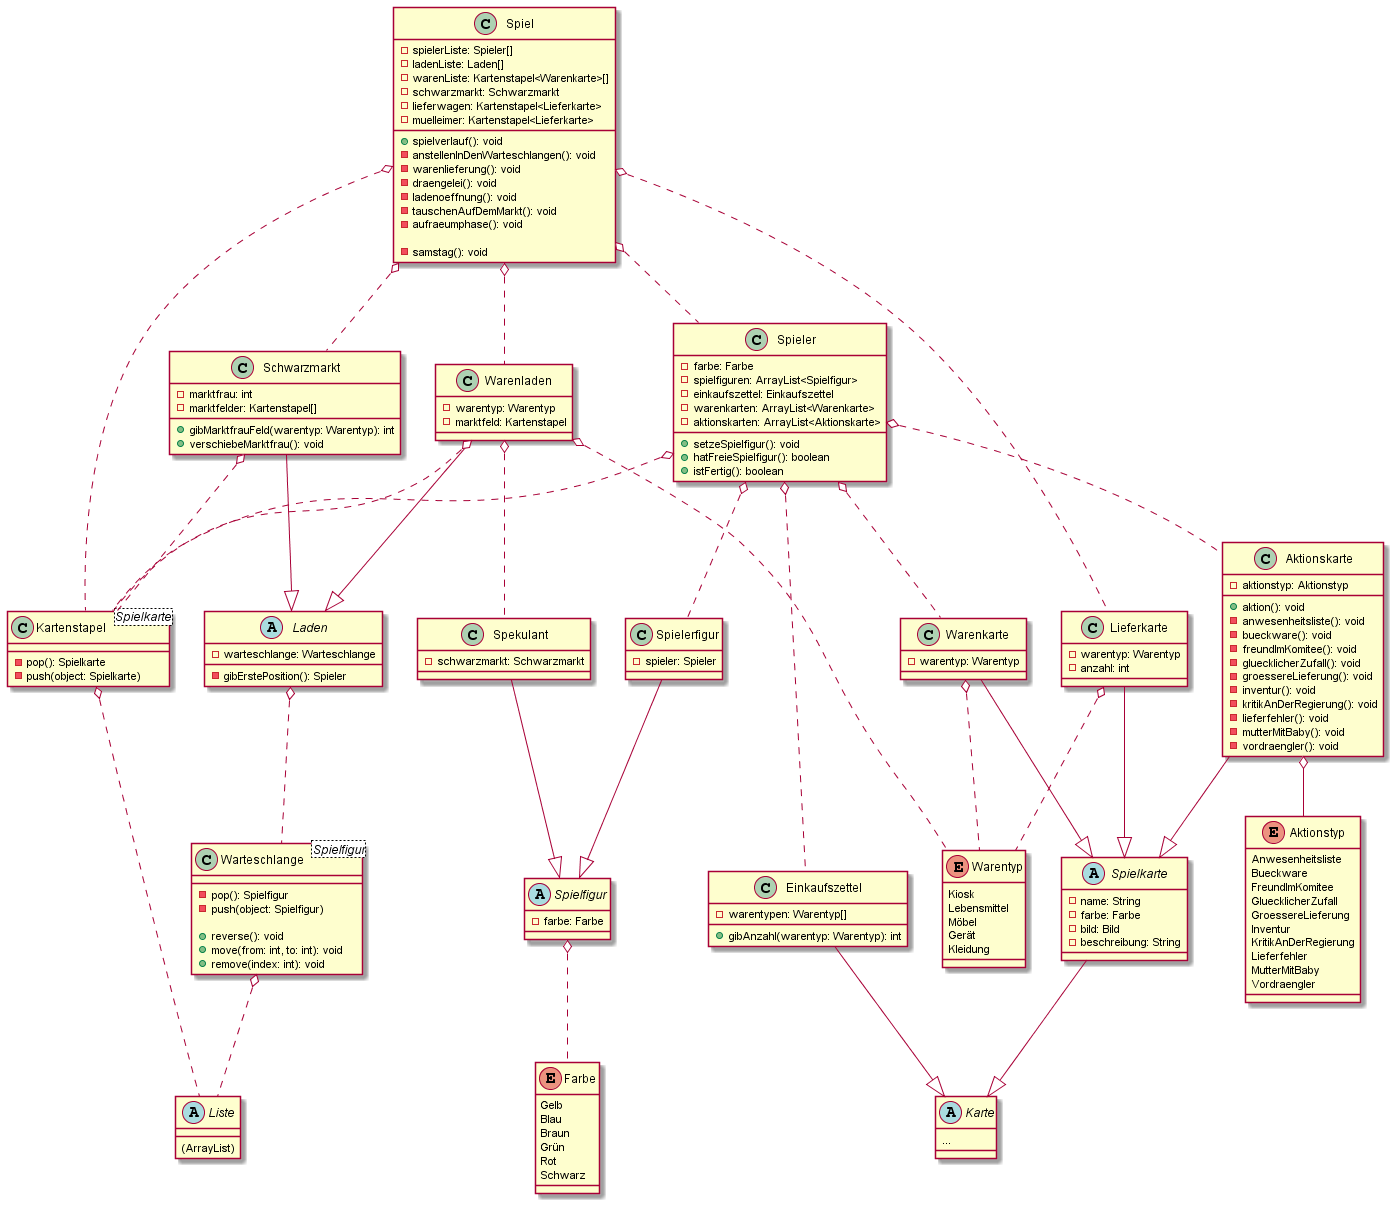
\includegraphics[width=1\textheight]{../../diagrams/out/classes/classes.png}
	\end{center}
\end{frame}

\begin{frame}
    \frametitle{Spiel}
    \begin{center}
        \begin{tikzpicture}
            \umlclass{Spiel}{
                -spielerListe:Spieler[]\\
                -ladenListe:Laden[]\\
                -warenListe:Kartenstapel<Warenkarte>[]\\
                -schwarzmarkt:Schwarzmarkt\\
                -lieferwagen:Kartenstapel<Lieferkarte>\\
                -muelleimer:Kartenstapel<Lieferkarte>\\ 
            }{
                +spielverlauf():void\\
                -anstellenInDenWarteschlangen():void\\  
                -warenlieferung():void\\
                -draengelei():void\\
                -ladenoeffnung():void\\
                -tauschenAufDemMarkt():void\\
                -aufraeumphase():void\\
                -samstag():void\\
            }
        \end{tikzpicture}
    \end{center}
\end{frame}

\begin{frame}
    \frametitle{Spieler}
    \begin{center}
        \begin{tikzpicture}
            \umlclass{Spieler}{
                -farbe:Farbe\\
                -spielfiguren:ArrayList<Spielfigur>\\
                -einkaufszettel:Einkaufszettel\\
                -warenkarten:ArrayList<Warenkarte>\\
                -aktionskarten:ArrayList<Aktionskarte>\\
            }{
                +setzeSpielfigur():void\\
                +hatFreieSpielfigur():boolean\\
                +istFertig():boolean\\
            }
        \end{tikzpicture}
    \end{center}
\end{frame}

\end{document}
